% Geometry taken directly from pg 1 of little moleskin theory book
\newcommand{\alat}{1 cm}
\newcommand{\sqth}{1.73205080757}
\newcommand{\Klen}{2 cm}
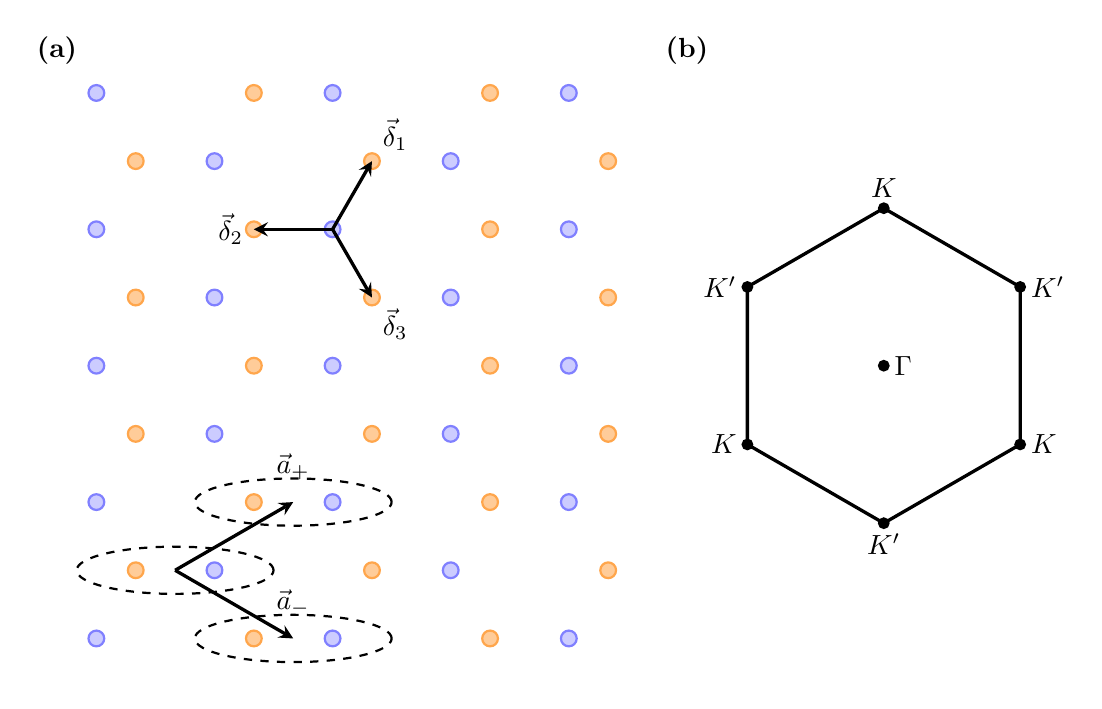
\begin{tikzpicture}															

	% Graphene lattice, sublattices different colors, nearest neighbor vectors and lattice vectors
	\begin{scope}[xshift=-3.5 cm,>=stealth,
		nnarrow/.style={color=black,very thick, ->},					% Nearest neighbor vectors
		A/.style={circle,draw=blue!50,fill=blue!20,
			thick,minimum size=2 mm,inner sep=0pt}, 					% A sublattice dots
		B/.style={circle,draw=orange!70,fill=orange!40,
			thick,minimum size=2mm,inner sep=0pt},						% B sublattice dots
		el1/.style={x radius=1.25*\alat,y radius=.3*\alat},				% Style for the ellipse
		el2/.style={dashed,thick}]										% Style for the ellipse draw

		%This scope is clipped to limit the drawn lattice to a square
		\clip (-3.5cm,-4cm) rectangle(4cm,4cm);
		% Draw the lattice
		\foreach \ip in {-3,-2,...,3}
			\foreach \im in {-3,-2,...,3}
			{
			\node at (\ip*\alat*3/2+\im*\alat*3/2      ,\ip*\sqth*\alat/2-\im*\sqth*\alat/2) [A] {};
			\node at (\ip*\alat*3/2+\im*\alat*3/2-\alat,\ip*\sqth*\alat/2-\im*\sqth*\alat/2) [B] {};
			}

		% Draw the nearest neighbor vectors
		\draw[nnarrow] (0,\alat*\sqth) -- +(60 :\alat) node[anchor=south west]{$\vec{\delta}_1$};
		\draw[nnarrow] (0,\alat*\sqth) -- +(180:\alat) node[anchor=east      ]{$\vec{\delta}_2$};
		\draw[nnarrow] (0,\alat*\sqth) -- +(-60:\alat) node[anchor=north west]{$\vec{\delta}_3$};
		
		% Draw the lattice vectors
		\draw[nnarrow] (240:3*\alat) ++(-\alat/2,0) -- +( 30:\sqth*\alat) node[circle,anchor=south]{$\vec{a}_+$};
		\draw[nnarrow] (240:3*\alat) ++(-\alat/2,0) -- +(-30:\sqth*\alat) node[circle,anchor=south]{$\vec{a}_-$};

		% Ellipses around two atom basis
		\draw[el2] (240:3*\alat) ++(-\alat/2,0) +(  0,0          ) ellipse[el1];
		\draw[el2] (240:3*\alat) ++(-\alat/2,0) +( 30:\sqth*\alat) ellipse[el1];
		\draw[el2] (240:3*\alat) ++(-\alat/2,0) +(-30:\sqth*\alat) ellipse[el1];
	\end{scope}

	% Reciprocal space BZ and high symmetry points
	\begin{scope}[xshift=3.5cm,
		BZ/.style={color=black,fill=black,very thick},
		circ2/.style={radius=1.5pt}]

		% Draw the BZ
		\draw[BZ]
			( 30:\Klen) circle[circ2] node[anchor=west] {$\bm{K'}$} --
			( 90:\Klen) circle[circ2] node[anchor=south]{$\bm{K}$}  --
			(150:\Klen) circle[circ2] node[anchor=east] {$\bm{K'}$} -- 
			(210:\Klen) circle[circ2] node[anchor=east] {$\bm{K}$}  -- 
			(270:\Klen) circle[circ2] node[anchor=north]{$\bm{K'}$} -- 
			(330:\Klen) circle[circ2] node[anchor=west] {$\bm{K}$}  -- 
			( 30:\Klen);

		% Label the high symmetry points
		\draw[BZ] (0,0) circle[circ2] node[anchor=west]{$\Gamma$};
	\end{scope}

	% (a) and (b) labels
	\node at (-7cm,4cm) {\textbf{(a)}};
	\node at ( 1cm,4cm) {\textbf{(b)}};
\end{tikzpicture}